%% The union API: what an algorithm says, and what the platform does with it.
%% Layout: three fixed columns, forward path along the top, return path along
%% the bottom on its own clear track — nothing shares a lane with anything.
\documentclass[tikz,border=4pt]{standalone}
\usepackage{xcolor}
%% Shared look for the UnionLabs system figures. \input by each fig-*.tex so a
%% colour or a corner radius is changed in one place.
\usetikzlibrary{positioning,arrows.meta,fit,backgrounds,calc}

\definecolor{uCode}{HTML}{1F6F5C}     % the experimenter's own code
\definecolor{uApi}{HTML}{6B4BA8}      % the contract / ARQ layer
\definecolor{uPhy}{HTML}{2E5E9E}      % transports / DSP
\definecolor{uRadio}{HTML}{B4700F}    % hardware
\definecolor{uShare}{HTML}{8A2E4D}    % the shared workspace

\tikzset{
  blk/.style={draw, rounded corners=2pt, align=center, font=\small,
              minimum height=8mm, inner sep=3pt, fill=black!2},
  code/.style={blk, draw=uCode, thick, fill=uCode!6},
  api/.style={blk, draw=uApi, very thick, fill=uApi!7},
  phy/.style={blk, draw=uPhy, thick, fill=uPhy!6},
  radio/.style={blk, draw=uRadio, thick, fill=uRadio!8},
  share/.style={blk, draw=uShare, thick, fill=uShare!6},
  stage/.style={blk, minimum height=9.5mm, font=\scriptsize, text width=16mm,
                inner sep=2pt},
  flow/.style={-{Latex[length=2mm]}, thick},
  back/.style={-{Latex[length=2mm]}, thick, densely dashed},
  % labels that sit ON an arrow: opaque, so the line never strikes the text
  onarrow/.style={font=\scriptsize\itshape, fill=white, inner sep=1.5pt},
  lbl/.style={font=\scriptsize\itshape, inner sep=1pt},
  note/.style={font=\scriptsize, align=left, inner sep=1pt},
  legend/.style={draw, minimum width=3mm, minimum height=3mm, inner sep=0pt},
}
\newcommand{\mono}[1]{{\ttfamily\footnotesize #1}}
\newcommand{\monos}[1]{{\ttfamily\scriptsize #1}}

\begin{document}
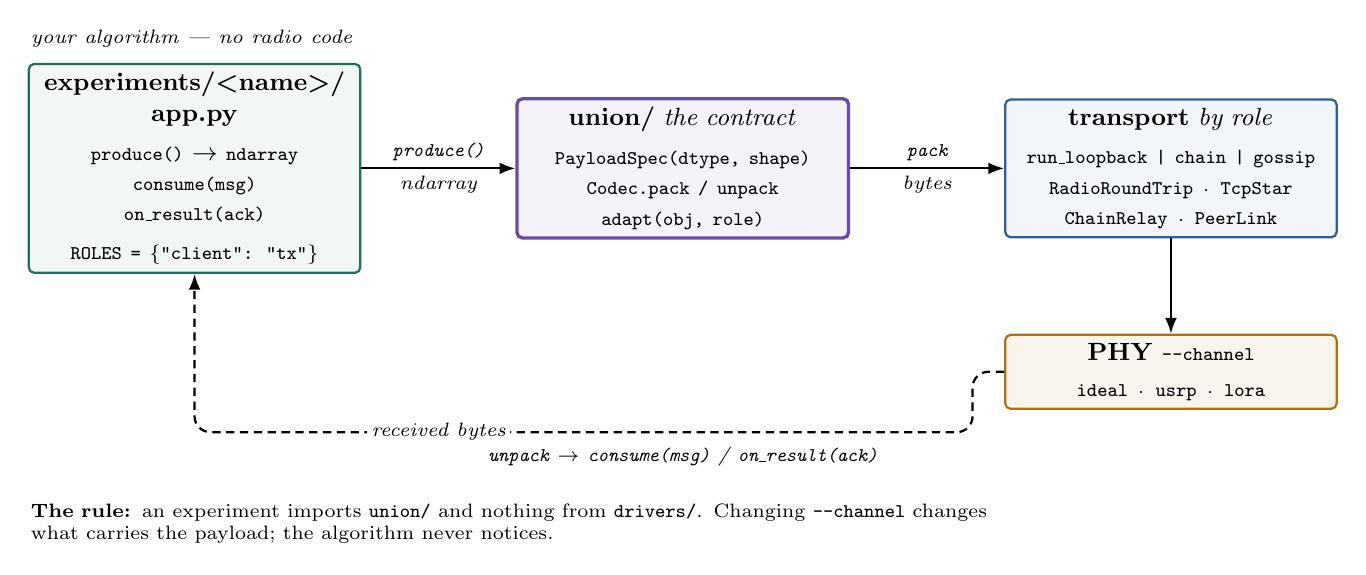
\begin{tikzpicture}

%% ── three columns on fixed coordinates ────────────────────────────────────
\node[code, text width=40mm] (app) at (0,0)
  {\textbf{experiments/\textless name\textgreater/}\\
   \textbf{app.py}\\[3pt]
   \monos{produce()} $\rightarrow$ \monos{ndarray}\\
   \monos{consume(msg)}\\
   \monos{on\_result(ack)}\\[3pt]
   \monos{ROLES = \{"client": "tx"\}}};
\node[lbl, above=1.5mm of app.north west, anchor=south west]
  {your algorithm --- no radio code};

\node[api, text width=40mm] (api) at (6.2,0)
  {\textbf{union/} \emph{the contract}\\[3pt]
   \monos{PayloadSpec(dtype, shape)}\\
   \monos{Codec.pack / unpack}\\
   \monos{adapt(obj, role)}};

\node[phy, text width=40mm] (tr) at (12.4,0)
  {\textbf{transport} \emph{by role}\\[3pt]
   \monos{run\_loopback | chain | gossip}\\
   \monos{RadioRoundTrip · TcpStar}\\
   \monos{ChainRelay · PeerLink}};

\node[radio, text width=40mm, anchor=north] (phy) at (12.4,-2.1)
  {\textbf{PHY} \monos{--channel}\\[2pt]
   \monos{ideal · usrp · lora}};

%% ── forward path, along the top row ───────────────────────────────────────
\draw[flow] (app.east) -- node[onarrow, above=1pt] {\monos{produce()}}
                          node[onarrow, below=1pt] {ndarray} (api.west);
\draw[flow] (api.east) -- node[onarrow, above=1pt] {\monos{pack}}
                          node[onarrow, below=1pt] {bytes} (tr.west);
\draw[flow] (tr.south) -- (phy.north);

%% ── return path, along its own bottom track ───────────────────────────────
\coordinate (track) at (0,-3.35);
\draw[back, rounded corners=2mm]
  (phy.west) -- ++(-4mm,0) |- (track -| api.south)
  -- (track -| app.south) -- (app.south);
\node[onarrow] at ($(track)!0.5!(track -| api.south)$) {received bytes};
\node[lbl, below=1.5mm of {track -| api.south}, anchor=north]
  {\monos{unpack} $\rightarrow$ \monos{consume(msg)} / \monos{on\_result(ack)}};

%% ── the rule ──────────────────────────────────────────────────────────────
\node[note, text width=126mm, anchor=north west]
  at ([yshift=-4mm]current bounding box.south west)
  {\textbf{The rule:} an experiment imports \monos{union/} and nothing from
   \monos{drivers/}. Changing \monos{--channel} changes what carries the
   payload; the algorithm never notices.};

\end{tikzpicture}
\end{document}
